% Graphic for TeX using PGF
% Title: /home/maksim/Documents/Bbd/3_b/figures/klasifikatoriaus_apmokymas.dia
% Creator: Dia v0.97.2
% CreationDate: Thu May 31 00:47:27 2012
% For: maksim
% \usepackage{tikz}
% The following commands are not supported in PSTricks at present
% We define them conditionally, so when they are implemented,
% this pgf file will use them.
\ifx\du\undefined
  \newlength{\du}
\fi
\setlength{\du}{15\unitlength}
\ttfamily\small
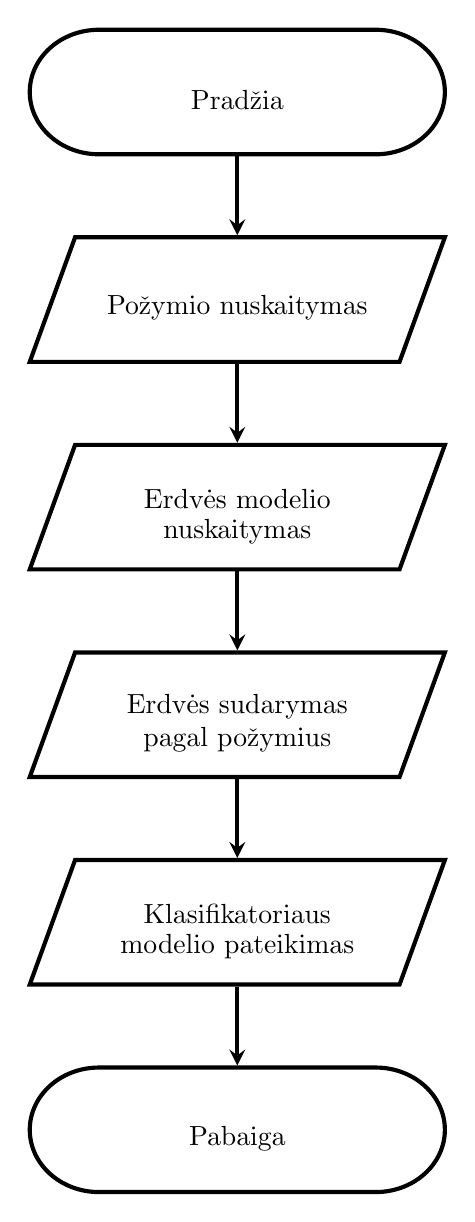
\begin{tikzpicture}
\pgftransformxscale{1.000000}
\pgftransformyscale{-1.000000}
\definecolor{dialinecolor}{rgb}{0.000000, 0.000000, 0.000000}
\pgfsetstrokecolor{dialinecolor}
\definecolor{dialinecolor}{rgb}{1.000000, 1.000000, 1.000000}
\pgfsetfillcolor{dialinecolor}
\definecolor{dialinecolor}{rgb}{1.000000, 1.000000, 1.000000}
\pgfsetfillcolor{dialinecolor}
\fill (21.091911\du,9.000000\du)--(30.000000\du,9.000000\du)--(28.908089\du,12.000000\du)--(20.000000\du,12.000000\du)--cycle;
\pgfsetlinewidth{0.100000\du}
\pgfsetdash{}{0pt}
\pgfsetdash{}{0pt}
\pgfsetmiterjoin
\definecolor{dialinecolor}{rgb}{0.000000, 0.000000, 0.000000}
\pgfsetstrokecolor{dialinecolor}
\draw (21.091911\du,9.000000\du)--(30.000000\du,9.000000\du)--(28.908089\du,12.000000\du)--(20.000000\du,12.000000\du)--cycle;
% setfont left to latex
\definecolor{dialinecolor}{rgb}{0.000000, 0.000000, 0.000000}
\pgfsetstrokecolor{dialinecolor}
\node at (25.000000\du,10.695000\du){Požymio nuskaitymas};
\pgfsetlinewidth{0.100000\du}
\pgfsetdash{}{0pt}
\pgfsetdash{}{0pt}
\pgfsetbuttcap
\pgfsetmiterjoin
\pgfsetlinewidth{0.100000\du}
\pgfsetbuttcap
\pgfsetmiterjoin
\pgfsetdash{}{0pt}
\definecolor{dialinecolor}{rgb}{1.000000, 1.000000, 1.000000}
\pgfsetfillcolor{dialinecolor}
\pgfpathmoveto{\pgfpoint{21.666667\du}{4.000000\du}}
\pgfpathlineto{\pgfpoint{28.333333\du}{4.000000\du}}
\pgfpathcurveto{\pgfpoint{29.253808\du}{4.000000\du}}{\pgfpoint{30.000000\du}{4.671572\du}}{\pgfpoint{30.000000\du}{5.500000\du}}
\pgfpathcurveto{\pgfpoint{30.000000\du}{6.328428\du}}{\pgfpoint{29.253808\du}{7.000000\du}}{\pgfpoint{28.333333\du}{7.000000\du}}
\pgfpathlineto{\pgfpoint{21.666667\du}{7.000000\du}}
\pgfpathcurveto{\pgfpoint{20.746192\du}{7.000000\du}}{\pgfpoint{20.000000\du}{6.328428\du}}{\pgfpoint{20.000000\du}{5.500000\du}}
\pgfpathcurveto{\pgfpoint{20.000000\du}{4.671572\du}}{\pgfpoint{20.746192\du}{4.000000\du}}{\pgfpoint{21.666667\du}{4.000000\du}}
\pgfusepath{fill}
\definecolor{dialinecolor}{rgb}{0.000000, 0.000000, 0.000000}
\pgfsetstrokecolor{dialinecolor}
\pgfpathmoveto{\pgfpoint{21.666667\du}{4.000000\du}}
\pgfpathlineto{\pgfpoint{28.333333\du}{4.000000\du}}
\pgfpathcurveto{\pgfpoint{29.253808\du}{4.000000\du}}{\pgfpoint{30.000000\du}{4.671572\du}}{\pgfpoint{30.000000\du}{5.500000\du}}
\pgfpathcurveto{\pgfpoint{30.000000\du}{6.328428\du}}{\pgfpoint{29.253808\du}{7.000000\du}}{\pgfpoint{28.333333\du}{7.000000\du}}
\pgfpathlineto{\pgfpoint{21.666667\du}{7.000000\du}}
\pgfpathcurveto{\pgfpoint{20.746192\du}{7.000000\du}}{\pgfpoint{20.000000\du}{6.328428\du}}{\pgfpoint{20.000000\du}{5.500000\du}}
\pgfpathcurveto{\pgfpoint{20.000000\du}{4.671572\du}}{\pgfpoint{20.746192\du}{4.000000\du}}{\pgfpoint{21.666667\du}{4.000000\du}}
\pgfusepath{stroke}
% setfont left to latex
\definecolor{dialinecolor}{rgb}{0.000000, 0.000000, 0.000000}
\pgfsetstrokecolor{dialinecolor}
\node at (25.000000\du,5.700000\du){Pradžia};
\definecolor{dialinecolor}{rgb}{1.000000, 1.000000, 1.000000}
\pgfsetfillcolor{dialinecolor}
\fill (21.091911\du,14.000000\du)--(30.000000\du,14.000000\du)--(28.908089\du,17.000000\du)--(20.000000\du,17.000000\du)--cycle;
\pgfsetlinewidth{0.100000\du}
\pgfsetdash{}{0pt}
\pgfsetdash{}{0pt}
\pgfsetmiterjoin
\definecolor{dialinecolor}{rgb}{0.000000, 0.000000, 0.000000}
\pgfsetstrokecolor{dialinecolor}
\draw (21.091911\du,14.000000\du)--(30.000000\du,14.000000\du)--(28.908089\du,17.000000\du)--(20.000000\du,17.000000\du)--cycle;
% setfont left to latex
\definecolor{dialinecolor}{rgb}{0.000000, 0.000000, 0.000000}
\pgfsetstrokecolor{dialinecolor}
\node at (25.000000\du,15.295000\du){Erdvės modelio};
% setfont left to latex
\definecolor{dialinecolor}{rgb}{0.000000, 0.000000, 0.000000}
\pgfsetstrokecolor{dialinecolor}
\node at (25.000000\du,16.095000\du){nuskaitymas};
\definecolor{dialinecolor}{rgb}{1.000000, 1.000000, 1.000000}
\pgfsetfillcolor{dialinecolor}
\fill (21.091911\du,19.000000\du)--(30.000000\du,19.000000\du)--(28.908089\du,22.000000\du)--(20.000000\du,22.000000\du)--cycle;
\pgfsetlinewidth{0.100000\du}
\pgfsetdash{}{0pt}
\pgfsetdash{}{0pt}
\pgfsetmiterjoin
\definecolor{dialinecolor}{rgb}{0.000000, 0.000000, 0.000000}
\pgfsetstrokecolor{dialinecolor}
\draw (21.091911\du,19.000000\du)--(30.000000\du,19.000000\du)--(28.908089\du,22.000000\du)--(20.000000\du,22.000000\du)--cycle;
% setfont left to latex
\definecolor{dialinecolor}{rgb}{0.000000, 0.000000, 0.000000}
\pgfsetstrokecolor{dialinecolor}
\node at (25.000000\du,20.295000\du){Erdvės sudarymas};
% setfont left to latex
\definecolor{dialinecolor}{rgb}{0.000000, 0.000000, 0.000000}
\pgfsetstrokecolor{dialinecolor}
\node at (25.000000\du,21.095000\du){pagal požymius};
\definecolor{dialinecolor}{rgb}{1.000000, 1.000000, 1.000000}
\pgfsetfillcolor{dialinecolor}
\fill (21.091911\du,24.000000\du)--(30.000000\du,24.000000\du)--(28.908089\du,27.000000\du)--(20.000000\du,27.000000\du)--cycle;
\pgfsetlinewidth{0.100000\du}
\pgfsetdash{}{0pt}
\pgfsetdash{}{0pt}
\pgfsetmiterjoin
\definecolor{dialinecolor}{rgb}{0.000000, 0.000000, 0.000000}
\pgfsetstrokecolor{dialinecolor}
\draw (21.091911\du,24.000000\du)--(30.000000\du,24.000000\du)--(28.908089\du,27.000000\du)--(20.000000\du,27.000000\du)--cycle;
% setfont left to latex
\definecolor{dialinecolor}{rgb}{0.000000, 0.000000, 0.000000}
\pgfsetstrokecolor{dialinecolor}
\node at (25.000000\du,25.295000\du){Klasifikatoriaus};
% setfont left to latex
\definecolor{dialinecolor}{rgb}{0.000000, 0.000000, 0.000000}
\pgfsetstrokecolor{dialinecolor}
\node at (25.000000\du,26.095000\du){modelio pateikimas};
\pgfsetlinewidth{0.100000\du}
\pgfsetdash{}{0pt}
\pgfsetdash{}{0pt}
\pgfsetbuttcap
\pgfsetmiterjoin
\pgfsetlinewidth{0.100000\du}
\pgfsetbuttcap
\pgfsetmiterjoin
\pgfsetdash{}{0pt}
\definecolor{dialinecolor}{rgb}{1.000000, 1.000000, 1.000000}
\pgfsetfillcolor{dialinecolor}
\pgfpathmoveto{\pgfpoint{21.666667\du}{29.000000\du}}
\pgfpathlineto{\pgfpoint{28.333333\du}{29.000000\du}}
\pgfpathcurveto{\pgfpoint{29.253808\du}{29.000000\du}}{\pgfpoint{30.000000\du}{29.671572\du}}{\pgfpoint{30.000000\du}{30.500000\du}}
\pgfpathcurveto{\pgfpoint{30.000000\du}{31.328428\du}}{\pgfpoint{29.253808\du}{32.000000\du}}{\pgfpoint{28.333333\du}{32.000000\du}}
\pgfpathlineto{\pgfpoint{21.666667\du}{32.000000\du}}
\pgfpathcurveto{\pgfpoint{20.746192\du}{32.000000\du}}{\pgfpoint{20.000000\du}{31.328428\du}}{\pgfpoint{20.000000\du}{30.500000\du}}
\pgfpathcurveto{\pgfpoint{20.000000\du}{29.671572\du}}{\pgfpoint{20.746192\du}{29.000000\du}}{\pgfpoint{21.666667\du}{29.000000\du}}
\pgfusepath{fill}
\definecolor{dialinecolor}{rgb}{0.000000, 0.000000, 0.000000}
\pgfsetstrokecolor{dialinecolor}
\pgfpathmoveto{\pgfpoint{21.666667\du}{29.000000\du}}
\pgfpathlineto{\pgfpoint{28.333333\du}{29.000000\du}}
\pgfpathcurveto{\pgfpoint{29.253808\du}{29.000000\du}}{\pgfpoint{30.000000\du}{29.671572\du}}{\pgfpoint{30.000000\du}{30.500000\du}}
\pgfpathcurveto{\pgfpoint{30.000000\du}{31.328428\du}}{\pgfpoint{29.253808\du}{32.000000\du}}{\pgfpoint{28.333333\du}{32.000000\du}}
\pgfpathlineto{\pgfpoint{21.666667\du}{32.000000\du}}
\pgfpathcurveto{\pgfpoint{20.746192\du}{32.000000\du}}{\pgfpoint{20.000000\du}{31.328428\du}}{\pgfpoint{20.000000\du}{30.500000\du}}
\pgfpathcurveto{\pgfpoint{20.000000\du}{29.671572\du}}{\pgfpoint{20.746192\du}{29.000000\du}}{\pgfpoint{21.666667\du}{29.000000\du}}
\pgfusepath{stroke}
% setfont left to latex
\definecolor{dialinecolor}{rgb}{0.000000, 0.000000, 0.000000}
\pgfsetstrokecolor{dialinecolor}
\node at (25.000000\du,30.700000\du){Pabaiga};
\pgfsetlinewidth{0.100000\du}
\pgfsetdash{}{0pt}
\pgfsetdash{}{0pt}
\pgfsetbuttcap
{
\definecolor{dialinecolor}{rgb}{0.000000, 0.000000, 0.000000}
\pgfsetfillcolor{dialinecolor}
% was here!!!
\pgfsetarrowsend{stealth}
\definecolor{dialinecolor}{rgb}{0.000000, 0.000000, 0.000000}
\pgfsetstrokecolor{dialinecolor}
\draw (25.000000\du,7.049072\du)--(25.000000\du,8.950928\du);
}
\pgfsetlinewidth{0.100000\du}
\pgfsetdash{}{0pt}
\pgfsetdash{}{0pt}
\pgfsetbuttcap
{
\definecolor{dialinecolor}{rgb}{0.000000, 0.000000, 0.000000}
\pgfsetfillcolor{dialinecolor}
% was here!!!
\pgfsetarrowsend{stealth}
\definecolor{dialinecolor}{rgb}{0.000000, 0.000000, 0.000000}
\pgfsetstrokecolor{dialinecolor}
\draw (25.000000\du,12.049072\du)--(25.000000\du,13.950928\du);
}
\pgfsetlinewidth{0.100000\du}
\pgfsetdash{}{0pt}
\pgfsetdash{}{0pt}
\pgfsetbuttcap
{
\definecolor{dialinecolor}{rgb}{0.000000, 0.000000, 0.000000}
\pgfsetfillcolor{dialinecolor}
% was here!!!
\pgfsetarrowsend{stealth}
\definecolor{dialinecolor}{rgb}{0.000000, 0.000000, 0.000000}
\pgfsetstrokecolor{dialinecolor}
\draw (25.000000\du,17.049072\du)--(25.000000\du,18.950928\du);
}
\pgfsetlinewidth{0.100000\du}
\pgfsetdash{}{0pt}
\pgfsetdash{}{0pt}
\pgfsetbuttcap
{
\definecolor{dialinecolor}{rgb}{0.000000, 0.000000, 0.000000}
\pgfsetfillcolor{dialinecolor}
% was here!!!
\pgfsetarrowsend{stealth}
\definecolor{dialinecolor}{rgb}{0.000000, 0.000000, 0.000000}
\pgfsetstrokecolor{dialinecolor}
\draw (25.000000\du,22.049072\du)--(25.000000\du,23.950928\du);
}
\pgfsetlinewidth{0.100000\du}
\pgfsetdash{}{0pt}
\pgfsetdash{}{0pt}
\pgfsetbuttcap
{
\definecolor{dialinecolor}{rgb}{0.000000, 0.000000, 0.000000}
\pgfsetfillcolor{dialinecolor}
% was here!!!
\pgfsetarrowsend{stealth}
\definecolor{dialinecolor}{rgb}{0.000000, 0.000000, 0.000000}
\pgfsetstrokecolor{dialinecolor}
\draw (25.000000\du,27.049072\du)--(25.000000\du,28.950928\du);
}
\end{tikzpicture}
